\section{Problem Definition}
\label{sec:pro}

In this part, we will introduce the problem we solve. To set the scene 
for this paper, we begin with the  \exref{ex-bear1} we mentioned
in \secref{sec:intro}. Assume that we have such kind of a repository,
which contains header files, body files and each file contains both source
code, i.e, {\it clock\_t get\_realtime(void)} and comments. In addition,
many commit messages are also created which touch many code files. Users
may insterested in what kind of semantic tags can be labeled to these
code files. Is it possible to build a computing taxonomy to classify
code files without large labeled code data?

We define the problem we want to tackle formally.
Assume $R=\left\{D,C,A\right\}$ is an entire code repository.
$D=\left\{d_1,..., d_N\right\}$ is the collection of all source code files of $R$, 
including all header files and body files. 
$C=\left\{c_1,..., c_U\right\}$ means all the commits that is created by programmers
for $R$.For each $c\in C$ a list of files $d \in D$ are touched by this commit.
For each $A=\left\{a_{i,j}\right\},0 \le i \le N,0 \le j \le U$ represent the many 
to many realtionships between code files and commits. For source code files, there are
two kinds of words. Let code identifiers $w_{i,d}^x$ be the $i$th 
observation in $d$ document and comment words $w_{j,d}^y$ be the $j$th 
observation in $d$ document. Let the size of the vocabulary be $V = N$.

The taxonomy $T=\left\{tags, E, P\right\}$ is a hierarchical graph.
$tags = \left\{tag_i\right\}$ means the tag set. $E=\left\{e_i\right\}$
evaluate the relatedness of two different tags. $P=\left\{tag_i, tag_j\right\},0 \le i,j \le T$
record the parent-child relationship of two different tags. 

Our problem is defined as follows:
\begin{Problem}
\label{pro:pro}
Given a code repository $R$ and a multi-labeled taxonomy system $T$, the problem is
For $d_i\in D \in R,0 \le i \le N$, to find the top-K possible $tag$ from the tags candidate $tags$.
\end{Problem}

This is kind of a multi-labeled classification problem. What we classify is code
repositories data. However, there is no labeled data for us to train. In this paper,
we figure this out by mining natural semanic features of the code data, which is the
main difference between this problem and the traditional multi-labeled classification problems.
\figref{fig:fram} shows the framework of our problem.
\begin{figure}[h]
\begin{center}
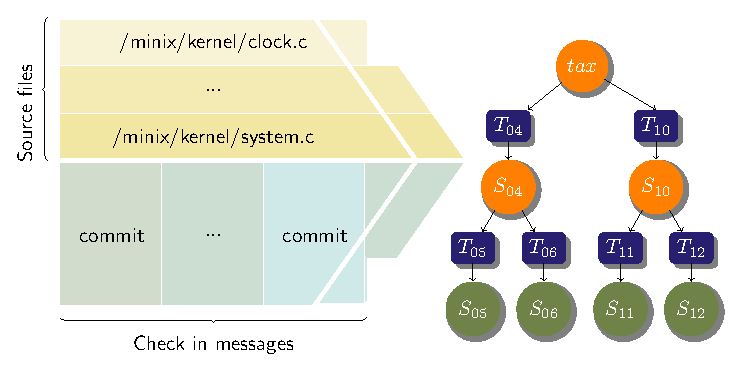
\includegraphics[width=\columnwidth]{figure/framework.eps}
\caption{Framework of code mining}
\label{fig:fram}
\end{center}
\end{figure}

We design a probabilistic graphical model for source code repositories. 
For taxonomy mapping,  we first set up a standarded taxonomy system and also apply different methods 
 to map a source code file to specific concept. We will refer to individual groups 
 of bag-of-word data as documents. 
